\documentclass[
    tikz,
    convert={outext=.svg, command=\unexpanded{pdf2svg \infile\space\outfile}},
    multi=false
]{standalone}
\usetikzlibrary{arrows, arrows.meta, automata, calc, fit, positioning, shapes}

\begin{document}
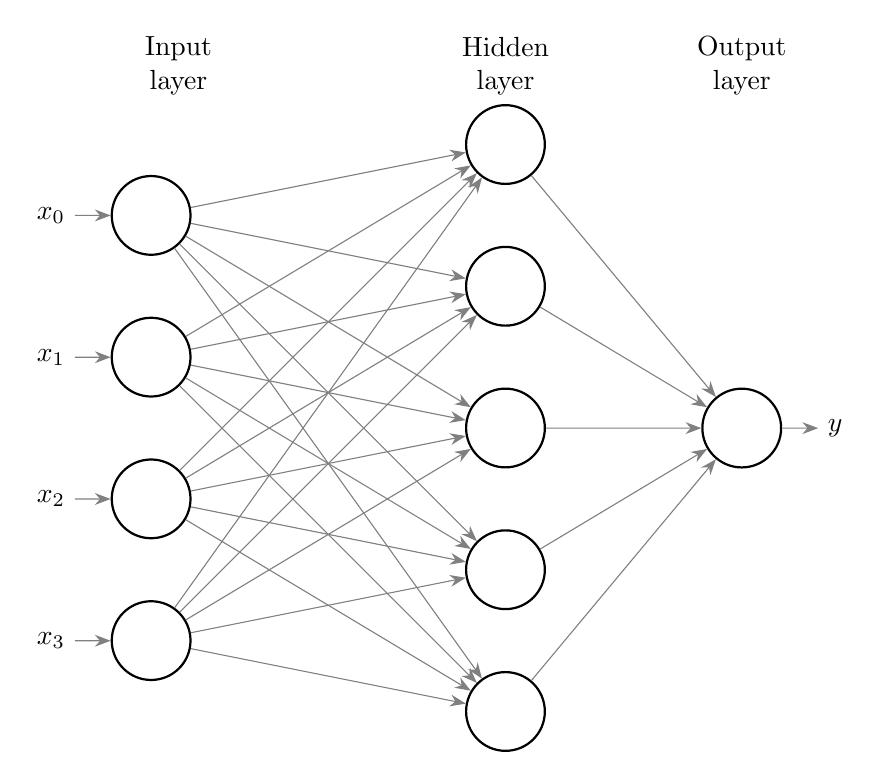
\begin{tikzpicture}[scale=1.8, >={Stealth[length=2mm]},->, draw=black!50, node distance=3cm]
    \tikzstyle{every pin edge}=[<-]
    \tikzstyle{neuron}=[draw, black, thick, circle, minimum size=1cm, inner sep=0pt]
    \tikzstyle{annot} =[text width=4em, text centered]

    % Draw the input layer nodes
    \foreach \name / \y in {0,...,3}
    \node[neuron, pin=left:{$x_\y$}] (I-\name) at (0,-\y-1) {};

    % Draw the hidden layer nodes
    \foreach \name / \y in {1,...,5}
    \path[yshift=0.5cm]
    node[neuron] (H-\name) at (2.5cm,-\y cm) {};

    % Draw the output layer node
    \node[neuron,pin={[pin edge={->}]right:{$y$}}, right of=H-3] (O) {};

    % Connect every node in the input layer with every node in the hidden layer.
    \foreach \source in {0,...,3}
    \foreach \dest in {1,...,5}
    \path (I-\source) edge (H-\dest);

    % Connect every node in the hidden layer with the output layer
    \foreach \source in {1,...,5}
    \path (H-\source) edge (O);

    % Annotate the layers
    \node[annot,above of=H-1, node distance=1cm] (hl) {Hidden layer};
    \node[annot,left=2.5cm of hl] {Input layer};
    \node[annot,right of=hl] {Output layer};
\end{tikzpicture}
\end{document}
